%%This is a very basic article template.
%%There is just one section and two subsections.
\documentclass[12pt]{elsarticle}

% \usepackage[utf8]{inputenc}
%\usepackage[T1]{fontenc}
\usepackage[english]{babel}
% \usepackage{microtype} % optional, for aesthetics
% \usepackage{tabularx} % nice to have
% \usepackage{booktabs} % necessary for style
\usepackage{graphicx}
\usepackage{subfigure}
\usepackage{hyperref}
\usepackage{rotating}

\hypersetup{breaklinks=true}

\journal{Information and Software Technology}


% 
% \jotdetails{
%     volume=0,
%     articleno=0,
%     year=2010
%     % doisuffix=jot.2011.10.1.a1,
% %     url={\githuburl}
% }

\begin{document}
\begin{frontmatter}

\title{Performance in Model Transformations: Experiments with ATL, QVT and
Mistral}
% \runningtitle{Performance in Model Transformations: Experiments with ATL and
% QVT}

\author[ut]{S.~Bosems\corref{cor1}}

\author[tue]{M.~van Amstel}
\author[ut]{I.~Kurtev}
\author[ut]{L.~Ferreira Pires}

\cortext[cor1]{Corresponding author}

\address[ut]{Faculty of Electrical Engineering, Mathematics and Computer
Science, University of Twente, Drienerlolaan 5, 7522NB, Enschede, The
Netherlands}
% The url of the MCS department is too long to fit on one line, so I needed this
% ugly fix to split it manually. Automatic splitting did not seem to work.
\address[tue]{Department of Mathematics and Computer Science, Eindhoven
University of Technology, Den Dolesch 2, 5612AZ, Eindhoven, The Netherlands}

\begin{abstract}
Model transformations are increasingly being incorporated in software development
processes. However, as systems being developed with transformations and models
grow in size and complexity, the performance of the transformations tends to
degrade. In this paper we investigate the factors that have an impact on the execution performance
of model transformations. We analyze the performance of three model
transformation language engines, namely ATL, QVT Operational Mappings, and Mistral. We implemented solutions to two transformation problems
in these languages, and compared the performance of these transformations.
Additionally, we implemented these transformations in Java in order to
evaluate the performance overhead imposed by the transformation languages. We extracted metric values from the transformations to systematically analyze how their 
characteristics influence transformation execution performance. In order to
evaluate the effect of language constructs on transformation performance, we
implemented different versions of the ATL and Mistral transformations
in functionally equivalent ways but using different strategies. 
The results of this paper enable a transformation designer to estimate beforehand the
performance of a transformation, and to choose among implementation alternatives to
achieve the best performance. In addition, transformation engine developers may find some
of our results useful in order to tune their tools for better performance.
\end{abstract}

\begin{keyword}model transformations, metamodeling, ATL, QVT, Mistral,
transformation languages, transformation execution performance\end{keyword}
\end{frontmatter}
%\sloppy
\section{Introduction}

Since the introduction of Model-Driven Engineering, model transformations have
become increasingly important in the software development process.
Transformations are applied to problems that potentially involve huge models
that need to be transformed. Examples of such problems are data translation and
interoperability, refactoring of large code bases and model extraction.
In order to be suitable for this task, transformation engines need to meet high
scalability and performance requirements. In addition, transformation developers need to know the factors that determine the performance
of transformations and need mechanisms to estimate and improve this performance.

Metamodels, models and transformation definitions all influence the
performance of model transformations. The size and complexity of
the input models are straightforward factors that affect transformation execution performance.
In some model transformation languages, a certain transformation problem can be solved
in multiple different but functionally equivalent ways. However, different
constructs may influence the transformation execution performance either positively
or negatively, and this needs to be investigated.

In this paper, we compare the performance of the transformation engines of three
languages: ATL \cite{jouault06}, QVT Operational Mappings \cite{qvt_spec} and
Mistral \cite{KurtevB04}. The comparison is based on two carefully chosen
example transformations that are executed for series of randomly generated input
models with an increasing number of model elements. For each input model, we
measured and compared the duration of the transformation execution. In addition
we also implemented these transformations in Java, in order to evaluate the
performance overhead imposed by the transformation languages. In order to
analyze the effect of different language constructs on the performance of the
transformation engines, we implemented one of the example transformations in
five different ways in ATL and in two different ways in Mistral. Two version of the
transformations have been implemented in Java (with and without SiTra
\cite{akehurst2006}). We extracted metric values from the transformation definitions and
analyzed the relation between these values and the performance results. This analysis should
enable transformation implementors to estimate the performance of a given
transformation, and to choose among alternative transformation languages (engines) and/or
transformation language constructs. The results of this study can also be used
by developers of transformation engines in order to improve the currently
available tools.

This paper is structured as follows. Section~\ref{sec:approach} discusses the
approach taken in this experiment. Section~\ref{sec:metrics} elaborates on
the metrics derived from the model transformations and their input.
Section~\ref{sec:results} gives the results of our model transformation
experiments. Section~\ref{sec:discussion} analyzes these results and draws some conclusions.
Section~\ref{sec:rel_work} discusses related work. Section~\ref{sec:conclusion}
gives our general conclusions and recommendations for future work.

\section{Approach}\label{sec:approach}

The goal of this work is to compare the performance of the chosen transformation
languages and their engines when facing input models of varying size and complexity,
especially models that contain hundreds of thousands model elements.
Transformation performance can be affected by several factors. In this paper we
address the following factors:

\begin{description}
\item[Size of input model.] As the number of input elements increases so does
the number of the elements that are potentially matched by rules. This results
in an increase of the elements to be transformed and in the overall execution
time. We performed transformations on a series of models with increasing number
of model elements.
\item[Structure of input model.] Models can be generally considered as graphs with a possibly
complex interconnected structure of model elements. Model complexity may cause
performance decrease, if complex navigation and matching needs to be done over a model. Some models may expose a simpler, tree-like structure. In order to study the impact of the structure of input models on transformations, we
executed transformations over models with both simpler (tree-like and linear) structure, and
more complex interconnection structures.
\item [Transformation strategy.] A given transformation problem may be solved
in multiple alternative ways in a single language. Generally, different solutions may
perform differently. We investigated the impact of the usage of different language
constructs for a single transformation problem by implementing and executing
five different but functionally equivalent solutions for the same
transformation problem in ATL, and two for Mistral.
\end{description}

\begin{sloppypar} %needed to prevent problems with the long names of the
%transformation languages
We compared the two model transformation tools that are part
of the Eclipse M2M project (ATLAS Transformation Language
(ATL) \cite{jouault08}, Query/View/Transformations Operational Mappings (QVTo)
\cite{qvt_spec}, and a QVT-like language called Mistral \cite{KurtevB04}. The
transformations implemented for these tools have also been compared with respect to performance with transformations
implemented in Java, giving us a good indication of the performance overhead of
using transformation languages.
\end{sloppypar}

% We performed two experiments: \emph{comparison of transformation engines} and \emph{comparison of
% different implementations in a single language} (ATL). Both experiments are described in the
% sequel.

\subsection{Experimental Setup}\label{sec:experimental_setup}


We implemented two transformations in each language: the SimpleClass2SimpleRDBMS transformation and the RSS2ATOM transformation, both taken from the ATL zoo \cite{atl_zoo}. The
input models in the SimpleClass2SimpleRDBMS transformation are graph-like class diagrams, while the input models
of the RSS2ATOM transformation are tree-like. In this way we can compare how the structure of input models
affects transformation execution performance.

\subsubsection*{SimpleClass2SimpleRDBMS Transformation}

The SimpleClass2SimpleRDBMS transformation is one of the classical examples of model transformations,
and has been implemented in many languages. This transformation takes a simplified
class diagram as input and transforms this to a relational database
model. The input model consists of \emph{packages} that contain zero or more
\emph{classes} with \emph{associations} between them. Classes can have zero or
more \emph{attributes}. Only classes that are marked as persistent are
transformed to tables. Methods and other constructs normally found in class
diagrams are not supported it this transformation. The resulting output model
consists of \emph{tables} that have \emph{columns}, \emph{primary keys} and \emph{foreign keys}.

For the SimpleClass2SimpleRDBMS transformation, 62 models were generated using Epsilon
\cite{epsilon}. About half of these models correspond to a general case scenario,
in which some of the input classes are not marked as persistent and therefore
are not transformed. The other models correspond to a worst case scenario, in which
all classes are persistent and thus have to be transformed. The input models differ in
the number of classes and the number of attributes per class. Attributes are restricted
in such a way that the type of an attribute cannot be the class in which the attribute is defined.

The model transformations implemented per transformation scenario are
functionally equivalent: the same input models are used for each transformation
implementation, and the output models are, with a slight alteration in the order
of the elements, identical.

The transformation was implemented in all three transformation languages (ATL,
QVTo and Mistral) and in Java. We ensured that the output models generated by
all transformations are identical. To be able to compare the languages, we tried
to use similar constructs wherever possible. For example, the matched rules in the
ATL transformation are encoded as mappings in QVTo.

\subsubsection*{RSS2ATOM Transformation}

Unlike the graph-like structure of the SimpleClass models, Really Simple
Syndication (RSS) models can be described as trees. An RSS model
contains one \emph{channel} (one root node), which in turn contains zero or more
\emph{item}s (child nodes). Consequently, an RSS model contains no cycles.
Items in an RSS model have certain properties, like a title, description, a category, and a
channel to which they belong.

The result of the RSS2ATOM transformation is a model with a similar
tree-like structure, but as an ATOM model. Like RSS, the ATOM model
consists of a single root node that contains \emph{entries}. An ATOM entry is
structured in the same way as the RSS item.

Similarly to the SimpleClass2SimpleRDBMS case, we implemented functionally
equivalent RSS2ATOM transformations in each language. The generated output models
are identical for each of the transformations for all of the input models.

\subsubsection*{Transformation Environment}

In our experiments, we used the following transformation engines:

\begin{description}
\item[ATL.] ATL plugin version 3.2.1.
\item[QVTo.] QVTo plugin version 3.1.0.
\item[Mistral.] Mistral version 0.9.
\end{description}

The plugins were run in a 64-bit Eclipse 3.7 SR1 Indigo environment, with 2GB of
memory allocated to it.

The Java implementations of the transformations were executed using Ant scripts
started from inside Eclipse without Virtual Machine forking, in order to allow a
fair comparison with the transformations that run in Eclipse.

We executed all these transformations on the 64-bit Java Virtual Machine version
1.7 build 1, running on Microsoft Windows 7 Professional (64-bit version).  The
computer system was equipped with a quad core Intel Core i7 920 CPU, running at
2.67 GHz, and 6 GB of RAM.

The transformations were executed with several input models with increasing
size. Transformations were run three times and the average time was
taken. We executed the RSS2ATOM transformations 100 times. There was no
significant difference in times for each run. The transformation execution
process considered in our experiments starts at the moment the first metamodels
are loaded and ends when the resulting model has been serialized.

\subsection{Transformation Implementations}

We implemented the SimpleClass2SimpleRDBMS transformation in ATL using different implementation strategies to study the effect
of different language constructs on the performance of the transformation.
We choose ATL to perform this experiment since it is a hybrid language that allows
several alternative functionally equivalent implementations. The five
alternative transformations entail the following changes:

\begin{sloppypar}%One paragraph of sloppy linebreaking, otherwise the word
% Class2Relational overflows into the margin
\begin{description}
\item[Initial implementation (Transformation $ATL$).] The initial implementation
is a declarative transformation that inlines the navigation code over the input
model in the bindings of transformation rules. It also uses the OCL operation
\texttt{allInstances()} in order to obtain instances of class Association.
\item[Move navigation to attribute helpers (Transformation $ATL_a$).] In this transformation we moved the navigation
expressions from the bindings to ATL attribute helpers. This causes the
transformation to execute the navigation once, after which the result is cached
for reuse. We expected that the performance should improved due to the reduced
number of traversals over attributes of the classes.
\item[Remove \texttt{allInstances()} (Transformation $ATL_b$).] This transformation
replaced \texttt{allInstances()} operation over associations with a matched rule. In this
way each association is processed only once. Again, we expected an increased
performance due to the lower number of visits for a single association.
\item[Replace two matched rules with called rules (Transformation
$ATL_c$).] This transformation is hybrid since it contains both called and
matched (lazy) rules. We replaced two matched rules from $ATL_b$ with their
functionally equivalent called rules. Furthermore, the transformation does not
use the internal trace mechanism of declarative ATL when resolving classes to
tables.
\item[Implement imperatively (Transformation
$ATL_d$).] This transformation is purely imperative. It contains only called
rules with imperative blocks and does not use the trace mechanism. Tracing is
implemented by using a map-like structure available in ATL.
\end{description}
\end{sloppypar}

Transformations $ATL_c$ and $ATL_d$ are used to investigate the effect of mixing
imperative and declarative constructs in a single ATL transformation. Overall,
the five ATL transformations cover a wide spectrum of implementation options
ranging from pure declarative to pure imperative implementations.

The SimpleClass2SimpleRDBMS transformation was implemented in Mistral in two
different versions. We shall call these $Mistral$ and $Mistral_a$. Mistral is
a declarative unidirectional transformation language. It was first
reported in \cite{KurtevB04} and later on extended with reflective capabilities
\cite{Kurtev10}. After a recent significant improvement of the engine it was
possible to use the language in this experiment. Compared to ATL, Mistral offers
only two types of rules: model element rules and helper rules. Model element
rules are equivalent to matched rules in ATL with the possibility to
instantiate OCL structures in the rule target. Helper rules are equivalent to
ATL called rules. In contrast to ATL, Mistral allows modifications in both
the source and target models and navigation over the target models.

Transformation $Mistral$ uses \texttt{allInstances()} to process associations whereas
$Mistral_a$ uses a rule to process each association once. We expected that the
avoidance of \texttt{allInstances()} will lead to a better performance. Transformation
$Mistral$ is algorithmically equivalent to $ATL_a$, and $Mistral_a$ is
equivalent to $ATL_b$.

We implemented two versions of each transformation (SimpleClass2SimpleRDBMS and
RSS2ATOM) in Java, namely with and without SiTra~\cite{akehurst2006}. SiTra is a
library developed to facilitate the implementation of metamodel-based transformations in Java, offering facilities to define
and execute transformation rules. SiTra stores the execution traces of these
transformation rules, which avoids element duplication and allows one to
reach already transformed target elements from source elements. For our
SiTra-based version of our Java implementations we made some small adjustments
to the original SiTra code\footnote{from \url{http://www.cs.bham.ac.uk/~bxb/Sitra/download.html}} to
allow the use of the code generated from the metamodels with the Eclipse
Modeling Framework (EMF) tools~\cite{emf}.

\section{Metrics}\label{sec:metrics}

Software metrics have been extensively studied in the last
decades. \cite{Fenton1996} Metrics can be used to get quick insights into the
characteristics of a software artifact, among others. We have extracted metrics
from the ATL and the QVTo transformations by using the metrics collection tool
described in~\cite{Amstel2010_ATL} and~\cite{Amstel2010_metrics}, respectively.

In this section, we describe the characteristics of the different transformations
on the basis of the metrics extracted from the respective artifacts.
We have used these characteristics to explain differences in the performance of the transformations later on in Section~\ref{sec:discussion}.

\subsection{Java SimpleClass2SimpleRDBMS Transformations}

In the Java implementations the programmer has to keep track of the
order in which transformation rules are
executed. In the SiTra-based version, we implemented the
four inner transformation rules as specializations to the
{\small \texttt{Rule<Source,Target>}} class provided by the library, while
the high-level transformation controls the execution of these rules.

The Java implementation without SiTra has been strongly inspired by the SiTra
version in terms of structure with one class for each transformation rule.
However, in this implementation only tracing of the transformation from classes
to tables is maintained (as a {\small \texttt{HashMap<Class,Table>}}), since
this is the only tracing information necessary to perform the transformation.
This has reduced considerably the overhead imposed by SiTra, which has an
expensive tracing mechanism.

We refrain from giving an extensive account of the metrics of the Java
implementations, since they cannot be compared with transformations implemented
using transformation languages.


\subsection{ATL SimpleClass2SimpleRDBMS Transformations}
Table~\ref{tab:metrics:ATL:C2R} shows the metric values that were extracted from
the different ATL implementations for the SimpleClass2SimpleRDBMS
transformation. For the metrics that require aggregation, we used the mean. An
example of a metric requiring aggregation is \emph{number of elements per output
pattern}. The value we used in the analysis represents thus the mean number of
elements in all output patterns.\\

\begin{table}[htb]
\centering\small
\begin{tabular}{|l|c|c|c|c|c|c|}
\hline
Metric & $ATL$ & $ATL_a$ & $ATL_b$ & $ATL_c$ & $ATL_d$ \\
\hline
\# Transformation rules & 4 & 4 & 4 & 6 & 7 \\
\hline
\# Matched rules & 4 & 4 & 4 & 1 & 0 \\
\hline
\# Non-lazy matched rules & 1 & 1 & 2 & 0 & 0 \\
\hline
\# Lazy matched rules & 3 & 3 & 2 & 1 & 0 \\
\hline
\# Called rules & 0 & 0 & 0 & 5 & 7 \\
\hline
\# Rules with an input filter & 1 & 1 & 2 & 0 & 0 \\
\hline
\# Rules with a \texttt{do}-section & 0 & 0 & 1 & 5 & 7 \\
\hline
\# Helpers & 0 & 2 & 1 & 2 & 2 \\
\hline
\# Attribute helpers & 0 & 2 & 1 & 2 & 2 \\
\hline
\# Operation helpers & 0 & 0 & 0 & 0 & 0 \\
\hline
\# Calls to \texttt{resolveTemp()} & 0 & 0 & 2 & 0 & 0 \\
\hline
\# Calls to \texttt{allInstances()} & 1 & 1 & 0 & 2 & 2 \\
\hline
\# Calls to built-in functions & 10 & 10 & 11 & 17 & 22 \\
\hline
\# Elements per output pattern & 1 & 1 & 1 & 0,67 & 0,57 \\
\hline
\# Parameters per called rule & 0 & 0 & 0 & 0,8 & 0,86 \\
\hline
\# Statements per \texttt{do}-section & 0 & 0 & 1 & 1,4 & 1,43 \\
\hline
\# Bindings per rule & 2,5 & 2,5 & 2,5 & 1,67 & 1,43 \\
\hline
Avg.\ helper cyclomatic complexity & 0 & 1 & 1 & 1 & 1 \\
\hline
\# Operations on collections per helper & 0 & 1 & 1 & 1 & 1 \\
\hline
\# Operations on collections per rule & 6 & 4 & 3,33 & 2,8 & 2,8 \\
\hline
%\# Calls to (Lazy Matched and Called) Rules per Rule (Fan-In) & 2 & 2 & 2,5 & 1,33 & 1,29 \\
%\hline
\# Avg.\ rule fan-in & 1,5 & 1,5 & 1,25 & 1,33 & 1,29 \\
\hline
\# Avg.\ helper fan-in & 0 & 3 & 5 & 5 & 7 \\
\hline
\# Avg.\ rule fan-out & 1,5 & 3 & 2,5 & 3 & 3,29 \\
\hline
\# Avg.\ helper fan-out & 0 & 0 & 0 & 0 & 0 \\
\hline
\# Calls to \texttt{resolveTemp()} per rule & 0 & 0 & 0,5 & 0 & 0 \\
\hline
\# Calls to \texttt{allInstances()} per rule & 0,25 & 0 & 0 & 0,33 & 0,29 \\
\hline
\# Calls to \texttt{allInstances()} per helper & 0 & 0,5 & 0 & 0 & 0 \\
\hline
\end{tabular}
\normalsize
\caption{Metrics from the different ATL versions of the SimpleClass2SimpleRDBMS transformation}
\label{tab:metrics:ATL:C2R}
\end{table} 

The three declarative versions all consist of four transformation rules, whereas
the imperative versions require more rules. From an understandability point of
view, the declarative versions are preferred, since smaller transformations are
expected to be more understandable~\cite{Amstel2011_MtATL}. Obviously, only the
imperative versions of the transformation contain called rules. It is to be
expected that only the imperative transformations contain an (imperative)
\texttt{do}-section. However, also declarative transformation~$ATL_b$ contains a
\texttt{do}-section. The reason for this is that this version of the
transformation requires navigation of the target model, which is not possible in
declarative ATL. The \emph{number of elements per output pattern\/} is lower for
the imperative transformations, since some of the features of the target model
element are initialized in the \texttt{do}-section. From the metric \emph{number
of matched rules\/} can be derived that transformation~$ATL_d$ is indeed
completely imperative. The imperative implementations contain only non-lazy
matched rules and called rules. These implementations do not require an input
filter to restrict the matching of a rule, because the rules are only invoked on
the model elements they need to be invoked for and thus require no further
restrictions.

The initial implementation, i.e., transformation~$ATL$, contains no helpers. All
other implementations do contain helpers, which are all attribute helpers. This
is to be expected, since only the initial implementation has the navigation code
in-line and in the other implementation it is moved to attribute helpers. In
implementations~$ATL_b$, $ATL_c$, and~$ATL_d$, the \texttt{allInstances()}
operator over associations has been removed, which requires one helper less.
However, in implementations~$ATL_c$, and~$ATL_d$ an extra attribute helper is
required to implement the map-like structure for tracing. One of the differences
between the initial implementation and the implementation where the navigation
is moved to attributes ($ATL_a$) is the number of calls to
\texttt{allInstances()}. From the metrics can be derived that they have been
moved from rules to helpers. The \texttt{allInstances()} function is used to
navigate a source model. Since navigation is the part that had been moved from
rules to helpers, this shift is to be expected.

\subsection{Mistral SimpleClass2SimpleRDBMS Transformations}

We do not have a set of standard metrics for Mistral language. The metrics from
the transformations are not necessary in our comparison since the only variation
is using (not using) of \texttt{allInstances()} OCL operation. The number of rules is quite
close to the number of rules in the transformations in other languages. Here are
some indicative numbers.

\begin{description}
\item[SimpleClass2SimpleRDBMS $Mistral$.] 1 model element rule, 3 helper rules.
\item[SimpleClass2SimpleRDBMS $Mistral_a$.] 2 model element rules, 3 helper
rules.
\item[RSS2ATOM.] 2 model element rules, 2 helper rules.
\end{description}

\subsection{QVTo Model Transformations}
Table~\ref{tab:metrics:QVTo} shows the metric values extracted from the QVTo model transformations.
Again, for the metrics that require aggregation we used the mean.\\

\begin{table}[htb]
\centering\small
\begin{tabular}{|l|c|c|}
\hline
Metric & SimpleClass2SimpleRDBMS & RSS2ATOM \\
\hline
\# Mappings & 5 & 7 \\
\hline
\# Mappings with condition & 1 & 0 \\
\hline
\# Helpers & 0 & 0 \\
\hline
\# Calls to \texttt{resolve} expressions & 6 & 0 \\
\hline
\# Elements per mapping & 68,8 & 43,86 \\
\hline
\# Parameters per mapping & 0 & 0 \\
\hline
\# Variables per mapping & 0,8 & 0 \\
\hline
\# Operations on collections per mapping & 1,4 & 0 \\
\hline
Cyclomatic complexity per mapping & 1 & 1 \\
\hline
\# Elements per helper & 0 & 0 \\
\hline
\# Parameters per helper & 0 & 0 \\
\hline
Cyclomatic Complexity per helper & 0 & 0 \\
\hline
Avg.\ mapping fan-in & 1,2 & 1,29 \\
\hline
Avg.\ helper fan-in & 0 & 0 \\
\hline
Avg.\ mapping fan-out & 0,6 & 1 \\
\hline
Avg.\ helper fan-out & 0 & 0 \\
\hline
Avg.\ \texttt{resolve} from mapping fan-in & 1,2 & 0 \\
\hline
\end{tabular}
\normalsize
\caption{Metrics from the QVTo transformations}
\label{tab:metrics:QVTo}
\end{table} 

The metrics show that both transformations are small. The
$Simple\-Class\-2\-Simple\-RDBMS$ transformation has slightly more complex
mappings, since they use conditions and consist of more sub-elements. Neither
transformation uses helpers. The $Simple\-Class\-2\-Simple\-RDBMS$
transformation uses operations on collections, whereas the \emph{RSS2ATOM} transformation does
not. Apart from this, the metrics sketch a similar picture for both
transformations. Also, the  metrics show that the sizes in terms of the number
of transformation functions of the QVTo implementations are similar to the sizes
of the ATL implementations.

\subsection{ATL RSS2ATOM Transformation}
Table~\ref{tab:metrics:ATL:R2A} shows the metric values that were extracted from
the ATL implementation of the RSS2ATOM transformation. Again, for the metrics
that require aggregation we used the mean.\\

\begin{table}[htb]
\centering\small
\begin{tabular}{|l|c|}
\hline
Metric & RSS2ATOM \\
\hline
\# Transformation rules & 7 \\
\hline
\# Matched rules & 7  \\
\hline
\# Non-lazy matched rules & 2 \\
\hline
\# Lazy matched rules & 5 \\
\hline
\# Called rules & 0 \\
\hline
\# Rules with an input filter & 0 \\
\hline
\# Rules with a \texttt{do}-section & 0 \\
\hline
\# Helpers & 0 \\
\hline
\# Attribute helpers & 0 \\
\hline
\# Operation helpers & 0 \\
\hline
\# Calls to \texttt{resolveTemp()} & 0 \\
\hline
\# Calls to \texttt{allInstances()} & 0 \\
\hline
\# Calls to built-in functions & 0 \\
\hline
\# Elements per output pattern & 1 \\
\hline
\# Parameters per called rule & 0 \\
\hline
\# Statements per \texttt{do}-section & 0 \\
\hline
\# Bindings per rule & 3,1 \\
\hline
Avg.\ helper cyclomatic complexity & 0 \\
\hline
\# Operations on collections per helper & 0 \\
\hline
\# Operations on collections per rule & 0 \\
\hline
%\# Calls to (Lazy Matched and Called) Rules per Rule (Fan-In) & 1,4 \\
%\hline
\# Avg.\ rule fan-in & 1 \\
\hline
\# Avg.\ helper fan-in & 0 \\
\hline
\# Avg.\ rule fan-out & 1 \\
\hline
\# Avg.\ helper fan-out & 0 \\
\hline
\# Calls to \texttt{resolveTemp()} per rule & 0 \\
\hline
\# Calls to \texttt{allInstances()} per rule & 0 \\
\hline
\# Calls to \texttt{allInstances()} per helper & 0 \\
\hline
\end{tabular}
\normalsize
\caption{Metrics from the ATL version of the RSS2ATOM transformation}
\label{tab:metrics:ATL:R2A}
\end{table} 

From the metrics can be concluded that the RSS2ATOM transformation is a very
small, completely declarative transformation.


\section{Results}\label{sec:results}

We executed the model transformations, and in this way we obtained the execution
time, measured in milliseconds, for each transformation and input model. With
these execution times, we discuss and justify the performance
differences of the transformations.

We first compare the different transformations using the
SimpleClass2SimpleRDBMS transformation, after which we look at the alternative
transformation strategies per language. Finally, we compare the different
transformations using the RSS2ATOM transformation.

\subsection{SimpleClass2SimpleRDBMS Transformations}

Figures~\ref{fig:attributes_compared} and \ref{fig:classes_compared}
compare the aspects of increasing the model size and complexity for different
transformation tools.\\

\begin{figure}[thb]
\centering
\subfigure[General case]{
\includegraphics[width=0.473\textwidth]{results/100attributes_compared_general}
\label{fig:100attributes_compared_general}
}
\subfigure[Worst case]{
\includegraphics[width=0.473\textwidth]{results/100attributes_compared_worst}
\label{fig:100attributes_compared_worst}
}
\caption{Comparison between transformations in ATL, using the
SimpleClass2SimpleRDBMS transformation (varying number of
classes)\label{fig:attributes_compared}}
\end{figure}

When increasing the size of the models, we observe a difference in performance
between the general and the worst case. Four out of five transformations
exhibit similar performances in both cases, however, the SiTra-based
implementation requires nearly five times as much time in the general case than
in the worst case for bigger models. This can be explained by considering the
input models and the structure of the SiTra-based implementation. For the general case scenario,
the models contain classes with some primary and non-primary attributes, and
some associations. A foreign key has to be created for each attribute that has
a type (Class) with at least one primary attribute, and for each association
between persistent classes in case the destination class has at least one
primary attribute. In the SiTra-based implementation, we perform queries to the
trace information to retrieve the tables corresponding to the classes that had
been generated before, and the SiTra package stores tracing information about
each object generated during a transformation. The mechanisms to perform
queries and store tracing information are not optimized in the SiTra
distribution, which explains the poor performance. In the worst case scenario,
the classes in the models have no primary attributes, therefore, these tracing
mechanisms are not executed, resulting in faster execution times.

\begin{figure}[thb]
\centering
\subfigure[General case]{
\includegraphics[width=0.478\textwidth]{results/100classes_compared_general}
\label{fig:100classes_compared_general}
}
\subfigure[Worst case]{
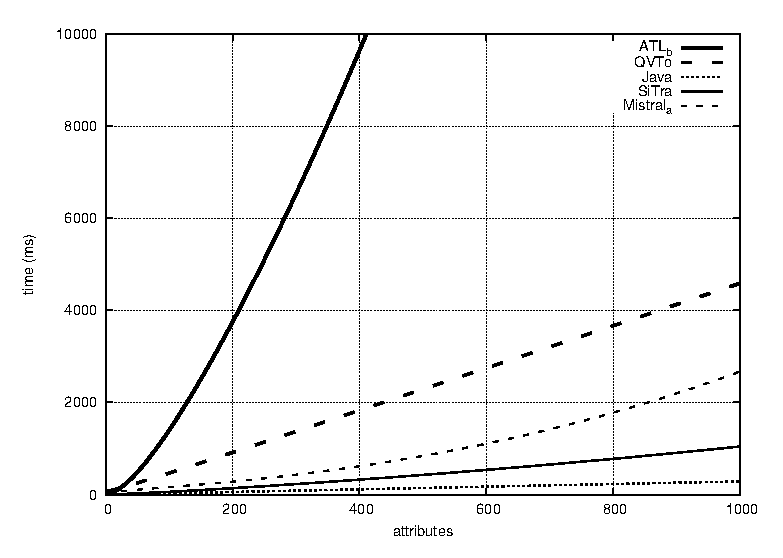
\includegraphics[width=0.478\textwidth]{results/100classes_compared_worst}
\label{fig:100classes_compared_worst}
}
\caption{Comparison between transformation tools, using the
SimpleClass2SimpleRDBMS transformation (varying number of attributes)
\label{fig:classes_compared}}
\end{figure}

If we increase the complexity of the models, as illustrated in
Figure~\ref{fig:classes_compared}, we see the same distribution of performance
among the different transformations. The decrease in performance is nearly the
same as when increasing the size of the input models. This is especially
apparent in case of SiTra. When comparing the general and the worst case
scenarios, we see that Java performs equally in either case. In the increased
model size scenario, Java performed slightly worse in the worst case.

\subsection{ATL SimpleClass2SimpleRDBMS Transformation
Implementations}\label{subsec:atl_class2relational}

Figures~\ref{fig:atl_attributes_compared} and \ref{fig:atl_classes_compared}
show the results obtained from running the different implementations of the
SimpleClass2SimpleRDBMS transformation in ATL.
Figure~\ref{fig:atl_attributes_compared} shows the results for transformations
run with input models with a fixed number of classes, and
Figure~\ref{fig:atl_classes_compared} shows the results of using input models
with a fixed number of attributes. The number of classes and attributes respectively
are fixed to 100.

In our experiment, we assumed that a model with more classes is
bigger, whereas a model containing more attributes and associations (with a
class as their type) are more complex, because each such attribute and
association actually defines a relation between classes. As such,
Figure~\ref{fig:atl_attributes_compared} shows the effect of increasing the
model complexity, whereas Figure~\ref{fig:atl_classes_compared}
shows the effect of increasing the model size.\\

\begin{figure}[thb]
\centering
\subfigure[General case]{
\includegraphics[width=0.478\textwidth]{results/atl_compared_general_100attributes}
\label{fig:atl_compared_general_100attributes}
}
\subfigure[Worst case]{
\includegraphics[width=0.478\textwidth]{results/atl_compared_worst_100attributes}
\label{fig:atl_compared_worst_100attributes}
}
\caption{Comparison between transformations in ATL, using the
SimpleClass2SimpleRDBMS transformation (varying number of
classes)\label{fig:atl_attributes_compared}}
\end{figure}

Figure~\ref{fig:atl_attributes_compared} shows that the implementation style of the
transformation indeed influences its performance. The two implementations that
exploit ATL's caching are, as expected, the fastest performing transformations, with little difference in
performance between them. The initial implementation is the third with regard to
performance.

By considering the results of the hybrid transformation ($ATL_c$), we
conclude that this implementation strategy had a negative impact on the
performance of the transformation as a whole. The purely imperative
transformation $ATL_d$ is the slowest one.\\

\begin{figure}[thb]
\centering
\subfigure[General case]{
\includegraphics[width=0.478\textwidth]{results/atl_compared_general_100classes}
\label{fig:atl_compared_general_100classes}
}
\subfigure[Worst case]{
\includegraphics[width=0.478\textwidth]{results/atl_compared_worst_100classes}
\label{fig:atl_compared_worst_100classes}
}
\caption{Comparison between transformations in ATL, using the
SimpleClass2SimpleRDBMS transformation (varying number of
attributes)\label{fig:atl_classes_compared}}
\end{figure}

Figure~\ref{fig:atl_classes_compared} shows a slightly different picture: the
size of the input models appears to have an impact on the performance of the
initial ATL implementation, which is now the second to worst performing
transformation. The order of the other transformations is unaffected.

\subsection{Mistral SimpleClass2SimpleRDBMS Transformation Implementations}

Figure~\ref{fig:mistral_attributes_compared} shows the performance of the
two Mistral transformations when increasing the number of classes, i.e. the
size of the model, with a fixed number of attributes.
Figure~\ref{fig:mistral_classes_compared} illustrates the effect of increasing
the number of attributes, i.e., the impact of an increasingly complex model.

\begin{figure}[thb]
\centering
\subfigure[General case]{
\includegraphics[width=0.478\textwidth]{results/mistral_compared_general_100attributes}
\label{fig:mistral_compared_general_100attributes}
}
\subfigure[Worst case]{
\includegraphics[width=0.478\textwidth]{results/mistral_compared_worst_100attributes}
\label{fig:mistral_compared_worst_100attributes}
}
\caption{Comparison between transformations in Mistral, using the
SimpleClass2SimpleRDBMS transformation (varying number of
classes)\label{fig:mistral_attributes_compared}}
\end{figure}

The elimination of \texttt{allInstances()} has a positive impact on the performance of
the Mistral transformation, as shown in
Figure~\ref{fig:mistral_attributes_compared}. In the general case, $Mistral_a$
is more than twice as fast as $Mistral$ as the models grow. In the worst case
scenario, $Mistral_a$ performs slightly worse than in the general case, however, $Mistral$ requires
over twice the time to complete the transformation for bigger models. This
result was expected, as running \texttt{allInstances()} over increasingly large models
were expected to impact the performance.

\begin{figure}[thb]
\centering
\subfigure[General case]{
\includegraphics[width=0.478\textwidth]{results/mistral_compared_general_100classes}
\label{fig:mistral_compared_general_100classes}
}
\subfigure[Worst case]{
\includegraphics[width=0.478\textwidth]{results/mistral_compared_worst_100classes}
\label{fig:mistral_compared_worst_100classes}
}
\caption{Comparison between transformations in Mistral, using the
SimpleClass2SimpleRDBMS transformation (varying number of
attributes)\label{fig:mistral_classes_compared}}
\end{figure}

Figure~\ref{fig:mistral_classes_compared} emphasizes that the complexity
increase of the models has little effect on the performance with regard to
implementation style. Both transformations perform similarly, with $Mistral_a$ performing slightly better.

\subsection{RSS2ATOM transformations}

Due to the tree structure of the input- and output models, we could not evaluate
the effect of model complexity, and general- and worst case scenarios for the
RSS2ATOM transformation. For similar reasons, no alternative of
transformation implementations have been created.

\begin{figure}[thb]
\centering
\includegraphics[width=0.478\textwidth]{results/rss2atom}
\caption{Transformation tools compared using the RSS2ATOM
transformation\label{fig:RSS2ATOM}}
\end{figure}

Figure~\ref{fig:RSS2ATOM} depicts the results obtained from the RSS2ATOM
experiment. Unlike the SimpleClass2SimpleRDBMS transformation,
the SiTra-based transformation is now the worst performing one for bigger
models. In the previous experiment, this transformation was the second best or
second worst performer, depending on the transformation scenario. As a result, ATL is now no longer the slowest tool. Our baseline
Java implementation is the fastest performing transformation, followed by
the Mistral transformation.

\subsection{Statistical Analysis}
To acquire more insights into the influence of the different implementation
strategies of the $SimpleClass2SimpleRDBMS$ transformation, we performed a
statistical analysis to relate the metrics presented in
Table~\ref{tab:metrics:ATL:C2R} with the performance results presented in
Section~\ref{subsec:atl_class2relational}. Therefore, we analyzed
correlations between the extracted metrics and the time it took to perform a
model transformation. Since we cannot assume that our data is distributed
normally, we use a non-parametric correlation test. In this case, we used
Spearman's rank correlation test. This test returns two values, viz.,
significance and correlation coefficient. The significance of the correlation
indicates the probability that there is no correlation between two variables
even though correlation is reported, i.e., the probability for a coincidence.
The correlation coefficient indicates the strength and direction of the
correlation. A positive correlation coefficient means that there is a positive
relation between metric and quality attribute and a negative correlation
coefficient implies a negative relation.


\paragraph{Declarative versus Imperative}
The main difference between the declarative and the imperative implementations
of the transformation is the use of matched rules versus the use of called
rules. Another difference is the use of \texttt{do}-sections in the imperative
version. Therefore, we analyzed the correlations between transformation time and
the metrics \emph{number of matched rules}, \emph{number of called rules}, and
\emph{number of rules with a \texttt{do}-section}. The results are shown in
Table~\ref{tab:cor:dec_vs_imp}.\\

\begin{table}[hbt] \centering\small
\begin{tabular}{|l|c|c|}
\cline{2-3}
\multicolumn{1}{c|}{}               & \multicolumn{2}{c|}{Transformation time}          \\
\cline{2-3}
\multicolumn{1}{c|}{}               & Correlation Coefficient & Significance (2-tailed) \\
\hline
\# Matched rules                    & -0,55 & 0,349  \\
\hline
\# Called rules                     & 0,55  & 0,349 \\
\hline
\# Rules with a \texttt{do}-section & 0,017 & 0,769 \\
\hline
\end{tabular}
\normalsize
\caption{Spearman correlations}
\label{tab:cor:dec_vs_imp}
\end{table}


The results show a negative correlation between the number of matched rules and
execution time. This means that more matched rules lead to a lower execution
time and thus better performance. The results show a positive correlation
between the number of called rules and \texttt{do}-sections, which indicates
that these constructs negatively affect performance. Unfortunately, the results
are not significant. A possible explanation for this is that there are too few
subjects in the analysis and that the differences among them are too small. This
may be solved by considering a larger transformation, where the differences are
larger and that allow for more hybrid implementations.

\paragraph{Moving Navigation to Attributes}
The main difference between the initial implementation and the the other ones,
where the navigation is moved to the attributes, is the number of attribute
helpers. Therefore, we analyzed the correlations between transformation time and
the metric \emph{number of attribute helpers}. The results are shown in
Table~\ref{tab:cor:mov_nav_to_attr}.\\

\begin{table}[tb] \centering\small
\begin{tabular}{|l|c|c|}
\cline{2-3}
\multicolumn{1}{c|}{}               & \multicolumn{2}{c|}{Transformation time}          \\
\cline{2-3}
\multicolumn{1}{c|}{}               & Correlation Coefficient & Significance (2-tailed) \\
\hline
\# Attribute helpers                & -0,13 & 0,830  \\
\hline
\end{tabular}
\normalsize
\caption{Spearman correlation}
\label{tab:cor:mov_nav_to_attr}
\end{table}


The results show a negative correlation between the number of attribute helpers
and execution time, meaning that using attributes has a beneficial effect on
performance. Similar to the declarative versus imperative case, the results are
not significant. This may be solved by considering hybrid implementations as
well, e.g., with only half of the navigation moved to attributes.


\paragraph{Usage of \texttt{allInstances()}}
In transformation $ATL_b$, the \texttt{allInstances()} operations have been removed.
Our expectation is that this is beneficial for performance.
Therefore, we analyzed the correlations between transformation time and the
metric \emph{number of calls to \texttt{allInstances()}}. The results are shown
in Table~\ref{tab:cor:allInst}.\\

\begin{table}[hbt]
\centering\small
\begin{tabular}{|l|c|c|}
\cline{2-3}
\multicolumn{1}{c|}{}               & \multicolumn{2}{c|}{Transformation time}          \\
\cline{2-3}
\multicolumn{1}{c|}{}               & Correlation Coefficient & Significance (2-tailed) \\
\hline
\# calls to \texttt{allInstances()} & 0,69 & 0,244  \\
\hline
\end{tabular}
\normalsize
\caption{Spearman correlation}
\label{tab:cor:allInst}
\end{table}

The results show a positive correlation between the number of calls to
\texttt{allInstances()}. This confirms our expectation that the use of the
\texttt{allInstances()} operations negatively affects performance. However,
again, it must be noted that the results are not significant. Also this may be
solved by considering hybrid implementations as well, e.g., with only half of
the calls to \texttt{allInstances()} removed.


\section{Discussion}\label{sec:discussion}

After obtaining the metrics from the model transformations and have
executed the transformations to gather performance data, we can analyze them in
order to find a correlation between metric values and the speed at which the
transformation can be run.

\subsection{Comparison of Transformation Implementations}

Comparing the different ATL transformations along each other, we see that the
relative difference does not change when either varying the number of classes
or the number of attributes. However, when looking at both these cases, we see
that when varying the number of classes, the $ATL$ transformation is the
third performing implementation, however, when varying the number of attributes,
this implementation is the second to last to finish executing. From this we can
conclude that the negative impact of increasing the complexity of the input
models is stronger than that of increasing their size for this specific
implementation.

In the results from our Mistral experiments we do not see a change in relative
results between the two implementations: the $Mistral_a$ implementation is the
fastest performer in any of the four scenario. What we can conclude from the
data, is that increasing the size of the models has a greater impact on the
$Mistral$ implementation, than increasing the complexity. This can be
explained when considering the number of calls to \texttt{allInstances()}: this is an
expensive method to use, and it is called more often and returns more results
when using more model elements. Since the number of model elements remains the
same when only increasing the complexity of the input models, the number of
calls to \texttt{allInstances()} remains unaltered, resulting in a better performance.

%%%%%%%%%%%%%%%%%%%%%%%%%%%%%%%%%%%%%%%%%%%%%%%%%%%%%%%%%%
% TODO: Discussion of performance with regard to metrics %
%%%%%%%%%%%%%%%%%%%%%%%%%%%%%%%%%%%%%%%%%%%%%%%%%%%%%%%%%%

\subsection{Comparison of Transformations}

The data shows that the pure Java implementation of the transformations is
indeed the fastest one. Depending on the input models, the SiTra-based
implementation may be the second performer, but can also be one of the slower
ones.

The performance of the Mistral transformation is less than that of Java, but
depending on the input models and thus the performance of the SiTra-based
implementation, it finishes either second or third.

The slowest performing transformation transformations are in ATL. An explanation
for this can be sought in the way the ATL engine works: the transformation
implementation is first compiled to an intermediate byte code form, which in turn
is interpreted by the ATL Virtual Machine. Furthermore, it has previously proved
that the ATL Virtual Machine has performance problems regarding collections.
\cite{cuadrado10}


\subsubsection*{QVT Relations}
As was the case in \cite{amstel2011}, we experimented with the QVT Relations
model transformation tool medini QVT \cite{mediniQVT} too. However, due to some
issues, the results of these transformations could not be incorporated in our
results.

Firstly, the medini QVT tool consists of an older 32-bit version of Eclipse
(3.5) bundled with the medini plugins. Since we executed the rest of the model
transformations on the latest version of Eclipse (3.7), the results would not
have been comparable.

Secondly, due to the working of medini\footnote{Every matched element is
printed to the console.}, the maximum amount of memory is allocated fast, even
for smaller models. This causes memory problems for the larger models, which can
thusly not be executed.

%%%%%%%%%%%%%%%%%%%%%%%%%%%%%%%%%%%%%%%%%%%%%%%%%%%%%%%%%%
% TODO: Discussion of performance with regard to metrics %
%%%%%%%%%%%%%%%%%%%%%%%%%%%%%%%%%%%%%%%%%%%%%%%%%%%%%%%%%%

\section{Related work}\label{sec:rel_work}

The basis for this work lies in~\cite{bosems2011} and \cite{amstel2011}. Here,
the model transformation tools ATL, QVT Operational Mappings and QVT Relations are
compared in a similar fashion as in this paper. The authors conclude that from
the three model transformation tools, ATL is the fastest performer, followed by
QVTo and QVTr. The difference with the current work is the environment in which
the transformations were run and which tools were used. In this paper we used
newer versions of the tools and a newer version of Java. Also, more memory was
allocated for the execution of the model transformations.

Transformation Tool Contest (TTC) \cite{toolcontest} is a series of events where
solutions to transformation problems are submitted and compared. The
transformation problems focus on various qualities, e.g. expressivity,
evolvability, performance, scalability and the ability of the tools to solve
certain problems, e.g. state space generation. The tool contest is a valuable
source of insight about the strong and weak points of transformation tools. However, there is still no clear focus of achieving real comparable results, statistical
soundness and relation to metrics over models and transformations. This event
can be considered as a potential host for well-defined experiments.

In~\cite{Amstel2009}, van Amstel et al.\ define quality attributes and metrics for
measuring them. Metrics are subdivided into size-, function-, module-, and consistency metrics.
The first deals with the size of the transformation, the second deals with the
complexity of functions, the third measures the complexity of modules as a
whole, the last measures covers the degree to which a transformation contains
conflicting information. Metrics from these four categories are related to
quality attributes and their effect, either positive or negative, is mentioned.
Understandability, modifiability, reusability, reuse, modularity, completeness,
consistency and conciseness are named as being of importance for the quality of
model transformations. The conclusion made by the authors is that the metrics
should be tested through an empirical study.

Based on the quality attributes defined by the previous work, \cite{vignaga09}
defines more metrics, divided into three categories: unit metrics, rule metrics
and helper metrics. The first contains the subcategories module metrics and
library metrics, the second covers matched rule, lazy matched rule and called
matched rule metrics, the last does not have any subcategories. In total, 81
metrics are defined. When comparing this set against the set of metrics defined
in \cite{Amstel2009}, the authors note that the difference in the number of
metrics can be explained by the size and complexity of the ATL metamodel, from
which the metrics were derived.

\section{Conclusions and Future Work}\label{sec:conclusion}

We presented a comparison of the performance of the execution engines of three
transformation languages: ATL, QVTo, and Mistral. Furthermore, we looked at
implementation of transformations using pure Java and a SiTra-based Java
implementation We studied how the size and complexity of the input models affect
the performance. Furthermore, we compared five different ATL transformations and
two different Mistral transformations that solve the same problem in order to
study the effect of different language constructs on the performance.

Overall, our pure Java implementation is the fastest among the transformations.
For the alternative ATL transformations we found that a declarative style
of implementing the transformation was the fastest, if calls to \texttt{allInstances()}
were avoided. This is also the case for the Mistral alternatives.

We provided metrics that can be used to measure how declarative an ATL
transformation is. These metrics can be used by transformation developers when
estimating the expected performance of a transformation. Our experiments run on
models of up to a million of elements and give an indication of the expected
time for the used transformations.

There are several works that define metrics over model transformation programs.
However, the research on how to relate basic metric values to more abstract and
complex transformation qualities is still in a very early phase.

Our work can be extended in several directions. We did not use metrics that
indicate how complex a model is. Our intuition is that a graph-like model is
more complex than a tree-like model. There are metrics for this characteristic
and they should be correlated with our results.

We ran our experiments on two toy-like examples. To obtain more realistic
results, the experiments should be repeated on real-life models that go beyond a
million of elements.

Not all the language features have been studied. For example, we could have
studied how usage of inheritance in ATL influences performance. The same is
valid for QVTo where navigation can be separated from the mappings by the means
of queries. In the experiments, all the rules contained simple source patterns.
It is well known that pattern matching is a complex operation. The effect of the
complexity of the source patterns needs to be studied.

The results reported in this paper are valid for the current versions of the
transformation engines. Alternative implementations may produce better results.
For example, some transformation engines are implemented as a compiler and
others as an interpreter. We believe that the results in this paper will be
useful to the language designers to improve the current state of their tools.

There are languages that are not covered in this paper. Our work should be
extended by covering more transformation languages.

\bibliographystyle{splncs03}
\bibliography{bibliography/references}

\end{document}
